%!TEX root = geometry.tex
\stepcounter{lecture}
\setcounter{lecture}{3}
\sektion{Möbius transformations}
\label{sec:m_bius_transformations}

\subsection{Stereographic projection} % (fold)
\label{sub:stereographic_projection}

\lecturemarker{8}{13 Feb}
We've encountered Möbius transformations before, in \emph{Groups}. These are transformations of the \emph{extended complex plane}, $\C\cup\{\infty\} = \C_\infty$. We'd like to consider how they apply to the sphere, $S^{\,2}$. To do this, first we need to map the sphere to the complex plane, which we do using \emph{stereographic projections}.

\begin{definition}
	Let $\NN=(0,0,1) \in S^2$ (the ``north pole''). Then we define the \emph{stereographic projection map} $\pi:S^{\,2}\backslash\{\NN\} \to \R^2 = \C$ by
	\begin{equation*}
		\pi(\pp) = \text{intersection of the Euclidean ray $\pp-\NN$ with the $x,y$ plane.}
	\end{equation*}
	Let's consider a slightly flattened picture of this: if $\pp=(x,0,z)$:

	\begin{center}
		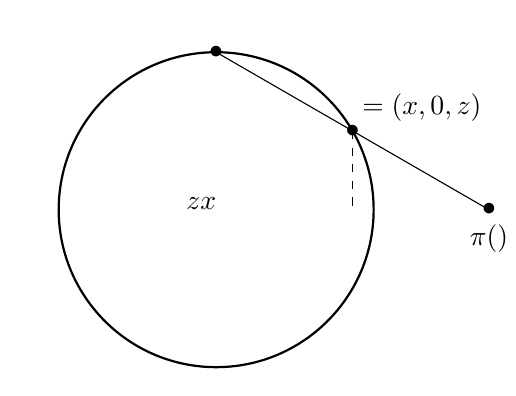
\begin{tikzpicture}[scale=2]

			\bigarrow (-1.3,0) -- (2.5,0) node [right=2pt] {$z$};
			\bigarrow (0,-1.3) -- (0,1.6) node [right] {$x$};

			\draw [thick] (0,0) circle (1);

			\draw (0,1) node [above left=2pt] {$\NN$} -- (1.732,0) node {$\bullet$};

			\draw (1.732,0) node [below=2pt] {$\pi(\pp)$};

			\draw (0,1) node {$\bullet$};
			\draw (30:1) node {$\bullet$};
			\draw (30:1) node [above right] {$\pp=(x,0,z)$};

			\draw [dashed] (30:1) -- ++ (0,-0.5);
		\end{tikzpicture}
	\end{center}
\end{definition}

This picture gives us a way to compute the value of $\pi(\pp)$ for a given point $\pp$. By considering the two similar triangles, we see that
\begin{equation*}
	\f{z}{1} = \f{\pi(\pp) - x}{\pi(\pp)} \implies \pi(\pp) = \f{x}{1-z},
\end{equation*}
and so the $x$-coordinate of $\pi(\pp)$ is $x/(1-z)$.

The projection is radially symmetric about the $z$-axis, and so by rotating, we have
\begin{equation*}
	\pi\left( (x,y,z) \right) = \f{x+iy}{1-z}.
\end{equation*}
So now we naturally ask how to invert the projection. In other words, given $w\iC$, can we find $\pp\in S^{\,2}$ with $\pi(\pp) = w$. We consider $w\iC$ with
\begin{equation*}
	w = \f{x+iy}{1-z}, \qquad x^2+y^2+z^2=1.
\end{equation*}
Squaring this equation gives
\begin{equation*}
	\left\vert w \right\vert^2
	= \f{x^2+y^2}{\left( 1-z^2 \right)^2}
	= \f{1-z^2}{\left( 1-z \right)^2}
	= \f{1+z}{1-z}.
\end{equation*}
We can solve this for $z$ in terms of $\left\vert w \right\vert$, which gives
\begin{equation*}
	z = \f{\left\vert w \right\vert^2-1}{\left\vert w \right\vert^2+1}
	\implies 1-z = \f{2}{\left\vert w \right\vert^2+1}.
\end{equation*}
Now we return to our definition of $w$. We have
\begin{equation*}
	x = \left( 1-z \right) \Re(w)
	\qqand
	y = \left( 1-z \right) \Im(w),
\end{equation*}
and thus we can write
\begin{equation*}
	\pi^{-1}(w) = \left( \f{2\,\Re(w)}{1+\left\vert w \right\vert^2}, \f{2\,\Im(w)}{1+\left\vert w \right\vert^2}, \f{\left\vert w \right\vert^2-1}{\left\vert w \right\vert^2+1} \right).
\end{equation*}
This will turn out to be a very useful formula.

This projection map does most of the work of identifying $\C_\infty$ to $S^{\,2}$. There are just two points left unaccounted for: $\infty\in\C_\infty$, and $\NN\in S^{\,2}$. It naturally follows that we can identify $\C_\infty$ and $S^{\,2}$ using the map
\begin{align*}
	w\iC & \longleftrightarrow \pi^{-1}(w) \in S^{\,2}, \\
	\infty & \longleftrightarrow \NN \in S^{\,2}.
\end{align*}
This tells us that $\{w_n\} \to \infty$ in $\C_\infty$ if and only if $\left\vert w_n \right\vert \to \infty$ also.

In this context, we call $\C_\infty$ the \emph{Riemann sphere}, and we will also encounter it in \emph{Complex Analysis} and \emph{Complex Methods}.

% We will encounter this in \emph{Complex Analysis} or \emph{Complex Methods}. A mereomophic fn is analogous to a holoc map $\C\to\C_\infty$.

% subsection stereographic_projection (end)

\subsection{Möbius group} % (fold)
\label{sub:m_bius_group}

Consider an invertible matrix
\begin{equation*}
	A=\mat{a & b \\c & d} \in \GL_2(\C).
\end{equation*}
This induces a Möbius map. We define
\begin{equation*}
	\fullfunction{\phi_A}{\C_\infty}{\C_\infty}{w}{\f{aw+b}{cw+d}},
\end{equation*}
with $\phi_A(-d/c)=\infty$ and $\phi_A(\infty) = a/c$.

% Thinking of Möbius maps as induced by matrices gives us some useful results:

\begin{lemma}
\mbox{}
\begin{enumerate}
	\shortskip
	\item $\phi_{\lambda A}(w)=\phi_A(w)$;
	\item $\phi_A(\phi_B(w)) = \phi_{AB}(w)$.
\end{enumerate}
\end{lemma}

\begin{proof}
	Part (i) is easy and left as an exercise. For (ii), define
	\begin{equation*}
		X = \left\{\ww\iC^2 : \ww\neq\bf{0}\right\}/\sim, \qquad \ww\sim\lambda\ww, \qquad \lambda\iC^*.
	\end{equation*}
	We can define a map $P:X\to\C_\infty$ by $P(w_1,w_2) = w_1/w_2$.

	Then $\GL_2(\C)$ acts on $X$ by $A\cdot\ww = A\ww$ (by matrix multiplication) and
	\begin{equation*}
		P(A\ww) = \phi_A(P(\ww)).
	\end{equation*}
	Then we have
	\begin{equation*}
		\phi_A(\phi_B(P(\ww)))
		= P(A \cdot (B \cdot \ww))
		= P(AB\ww)
		= \phi_{AB}(P(\ww)). \qedhere
	\end{equation*}
\end{proof}

It would have been easy to do this by simply plugging in matrices and turning the handle on some algebra, but this is a cleaner proof. It gives us some understanding of why the result is true.

	\pagebreak

\begin{corollary}
	We define the \emph{projective general linear group} as
	\begin{equation*}
		\PGL_2(\C) := \f{\GL_2(\C)}{\left\{\lambda I: \lambda\iC\right\}}.
	\end{equation*}
	This acts on $\C_\infty$.
\end{corollary}

\vspace{-3pt}

\begin{exercise}
	If $\SL_2(\C)$ is the special linear group, then show that
	\begin{equation*}
		\PGL_2(\C) = \f{\SL_2(\C)}{\left\{\pm I\right\}} =: \PSL_2(\C).
	\end{equation*}
\end{exercise}

\begin{definition}
	The \emph{Mobius group} is given by
	\begin{equation*}
		\Mobgp = \left\{\phi:\C_\infty \to \C_\infty: \phi(w)=\phi_A(w), A\in\GL_2(\C)\right\} \cong \PSL_2(\C).
	\end{equation*}
	Then $\phi\in\Mobgp$ is a \emph{Mobius transformation}. This is the group of all invertible holomorphic maps $\C_\infty \to \C_\infty$.
\end{definition}

\begin{lemma}
\mbox{}
\begin{enumerate}
	\item We can generate $\Mobgp$ with maps of the form
	\begin{itemize}
		\shortskip
		\item $z\mapsto az$, $a\iC^*$ (dilation);
		\item $z\mapsto z+b$, $b\iC$ (translation);
		\item $z\mapsto 1/z$ (inversion).
	\end{itemize}
	\item If $z_1,z_2,z_3$ and $w_1,w_2,w_3$ are two sets of distinct points in $\C_\infty$, then there is a unique $\phi\in\Mobgp$ with $\phi(z_i)=w_i$.
	\item \emph{Cross ratios.} If $z_1,z_2,z_3,z_4\iC_\infty$ are distinct and $\phi\in\Mobgp$ with $\phi(z_i)=w_i$, then cross ratios are preserved. That is,
	\begin{equation*}
		\f{\left( z_2-z_3 \right)\left( z_4-z_1 \right)}{\left( z_2-z_1 \right)\left( z_4-z_3 \right)}
		= \f{\left( w_2-w_3 \right)\left( w_4-w_1 \right)}{\left( w_2-w_1 \right)\left( w_4-w_3 \right)}.
	\end{equation*}
\end{enumerate}
\end{lemma}

\vspace{-6pt}

Proof is left as an exercise.

\begin{definition}
	Let $\cal{C}$ be the set of Euclidean lines and circles in $\C$.
\end{definition}

\begin{lemma}
	Let $S\subset\C$. Then $S\in\cal{C}$ if and only if $S$ satisfies an equation of the form \label{lem:eq-lines-circles}
	\begin{equation*}
		az\zbar + bz+\overline{bz}+c=0,
	\end{equation*}
	for $a,c\iR$, $b\iC$, and not all zero.
\end{lemma}

\begin{proof}
	A line satifies $\alpha x+\beta y = \gamma$, for $\alpha,\beta,\gamma\iR$, so
	\begin{equation*}
		\alpha\left( \f{z+\zbar}{2} \right) + \beta\left( \f{z-\zbar}{2i} \right) = \gamma.
	\end{equation*}
	Rearranging this gives
	\begin{equation*}
		\left( \f{\alpha-i\beta}{2} \right)z + \left( \f{\alpha+i\beta}{2} \right)\zbar = \gamma,
	\end{equation*}
	which is what we want.

	A circle satisfies $\left\vert z-p \right\vert^2=r^2$, so
	\begin{equation*}
		z\zbar-p\zbar-\overline{p}z+\left\vert p \right\vert^2 = r^2 \qquad \text{or} \qquad
		z\zbar-p\zbar-\overline{p}z+\left( \left\vert p \right\vert^2-r^2 \right) = 0,
	\end{equation*}
	which is again the desired form.

	The converse is very similar: if $a\neq 0$, then divide by $a$ and complete the square. If $a=0$, then we have a line. 
\end{proof}

\begin{corollary}
	If $S\in\cal{C}$, $\phi\in\Mobgp$, then $\phi(S)\in\cal{C}$. That is, Möbius maps takes lines and circles to lines and circles.
\end{corollary}

\begin{proof}
	It sufficies to check that this is true for the generators of $\Mobgp$.

	Take $w=\phi(z)=\alpha z$. If the equation of $S$ is $az\zbar + bz+b\zbar + c = 0$, then
	\begin{equation*}
		z = \alpha^{-1} w \implies
		\f{a}{\left\vert \alpha \right\vert^2}\,w\wbar + \f{b}{\alpha}\,w + \f{\overline{b}}{\overline{\alpha}}\,\wbar + c = 0.
	\end{equation*}
	This equation is of the same form, and so elements of $\cal{C}$ map to other elements of $\cal{C}$.

	The cases $z\mapsto z+b$ and $z\mapsto 1/z$ are similar. For the latter, the new equation is
	\begin{equation*}
		\f{a}{w\wbar} + \f{b}{w} + \f{\overline{b}}{\wbar} + c = 0 \implies a + b\wbar + cw\wbar = 0,
	\end{equation*}
	which is again of the same form.
\end{proof}

\begin{corollary}
	There's a unique element of $\cal{C}$ passing through any three distinct points $z_1,z_2,z_3\iC_\infty$.
\end{corollary}

\begin{proof}
	Choose $\phi\in\Mobgp$ with $\phi(z_1)=0$, $\phi(z_2)=1$ and $\phi(z_3)=2$. There's a unique line $S\in\cal{C}$ passing through $0,1,2$ in $\R$. So $C=\phi^{-1}(\R)$ is the set that we want.
\end{proof}

\begin{corollary}
	The group $\Mobgp$ acts transitively on $\cal{C}$.
\end{corollary}

\begin{proof}
	 Given $C_1,C_2$, pick $z_1,z_2,z_3$ on $C_1$, $w_1,w_2,w_3$ on $C_2$, and $\phi$ with $\phi(z_i) = w_i$. Then $\phi(C_1)$ passes though $w_1,w_2,w_3$, and so $\phi(C_1)=C_2$.
\end{proof}

\begin{examples}
\mbox{}
\begin{enumerate}
	\item If $\phi(z) = \df{z-i}{z+i}$, then $\phi(\R)=S^{\,1}\subset \C$.

	Consider: if $z\iR$, then $\left\vert z-i \right\vert = \left\vert z+i \right\vert = \sqrt{z^2+1}$.
	\item The stabiliser of the real line is given by
	\begin{equation*}
		A=\left\{\phi\in\Mobgp: \phi(\R)=\R\right\} = \left\{\phi_A: A\in\GL_2(\R)\right\}.
	\end{equation*}
	Similarly, the stabiliser of the circle has
	\begin{equation*}
		B
		= \left\{\phi\in\Mobgp: \phi(S^{\,1}) = S^{\,1}\right\}
		= \left\{\phi: \phi(z) = \lambda\,\f{z+\alpha}{\overline{\alpha}z+1}, \lambda\in S^{\,1}, \alpha\iC, |\alpha|^2\neq 1\right\}.
	\end{equation*}
	The idea of the proof is that $B=\phi A\phi^{-1}$, where $\phi$ is as in the previous example.
\end{enumerate}
\end{examples}

% subsection m_bius_group (end)